\documentclass[a4paper, 12pt]{article}
\usepackage[a4paper,top=1.5cm, bottom=1.5cm, left=1cm, right=1cm]{geometry}
\usepackage{cmap}					% поиск в PDF
\usepackage{mathtext} 				% русские буквы в формулах
\usepackage[T2A]{fontenc}			% кодировка
\usepackage[utf8]{inputenc}			% кодировка исходного текста
\usepackage[english,russian]{babel}	% локализация и переносы

\usepackage{amsmath}
\usepackage{indentfirst}
\usepackage{longtable}
\usepackage{graphicx}
\usepackage{array}

\usepackage{wrapfig}
\usepackage{siunitx} % Required for alignment
\usepackage{subfigure}
\usepackage{multirow}
\usepackage{rotating}
\usepackage{caption}

\graphicspath{{.}}


\title{\begin{center}Лабораторная работа №2.2.3\end{center}
Измерение теплопроводности воздуха при атмосферном давлении}
\author{Рожков А. В. \\ Преподаватель Яворский В. А.}
\date{\today}

\begin{document}
    \pagenumbering{gobble}
    \maketitle
    \newpage
    \pagenumbering{arabic}

    \textbf{Цель работы:} измерить коэффициент теплопроводности воздуха при атмосферном давлении в зависимости от температуры.

    \textbf{В работе используются:} цилиндрическая колба с натянутой по оси нитью; термостат ($\sigma_t = 0.1^o C$); вольтметр ($\sigma_U = 1~мВ$) и амперметр ($\sigma_I = 0.1~мА$); источник постоянного напряжения; магазин сопротивлений.

    \section{Теоретическая справка}

        \textit{Теплопроводность} — это процесс передачи тепловой энергии от нагретых частей системы к холодным за счёт хаотического движения частиц среды (молекул, атомов и т.п.). В газах теплопроводность осуществляется за счёт  непосредственной передачи кинетической энергии от быстрых молекул к медленным при их столкновениях. Перенос тепла описывается законом Фурье, утверждающим, что плотность потока энергии $\overline{q} = -k \nabla T$, где $k \left[ \dfrac{\text{Вт}}{\text{м} \cdot \text{К}} \right]$ - \textit{коэффициент теплопроводности}.

        Молекулярно-кинетическая теория дает следующую оценку для коэффициента теплопроводности газов:

        \begin{align}
            k &\sim \lambda \overline{\nu} \cdot n c_V \label{k}
        \end{align}

        С помощью некоторых преобразований мы получаем, что

        \begin{align}
            Q &= \dfrac{2 \pi L}{\ln \dfrac{r_0}{r_1}} k  \cdot \Delta T \label{Q}
        \end{align}


        \section*{Экспериментальная установка}
        \begin{wrapfigure}{r}{0.4\textwidth}
        \begin{center}
            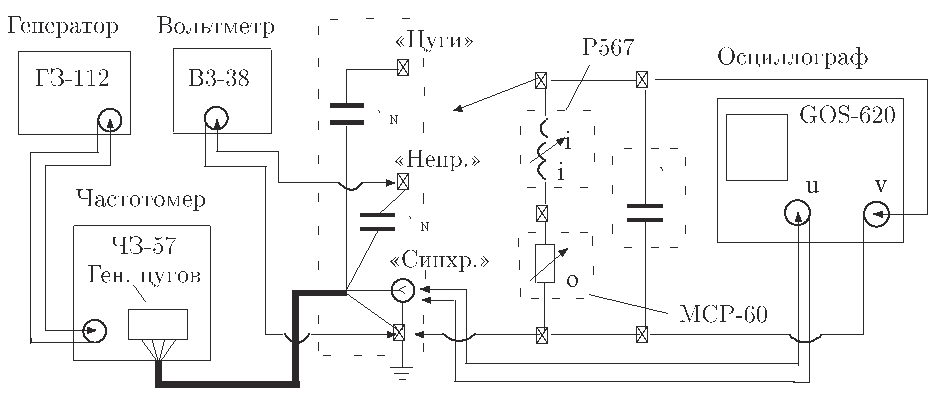
\includegraphics[width = 0.3\textwidth]{pictures/ustanovka.png}
        \end{center}
        \textbf{\caption{Схема установки}}
        \end{wrapfigure}
        Схема установки приведена на рис. 1. На оси полой цилиндрической трубки с внутренним диаметром $2r_0 \sim 1$ см размещена металлическая нить диаметром $2r_1 \sim 0,05$ мм и длиной $L \sim 40$ см (материал нити и точные геометрические размеры указаны в техническом описании установки). Полость трубки заполнена воздухом (полость через небольшое отверстие сообщается с атмосферой). Стенки трубки помещены в кожух, через которых пропускается вода из термостата, так что их температура $t_0$ поддерживается постоянной. Для предотвращения конвекции трубка расположена вертикально.

        Металлическая нить служит как источником тепла, так и датчиком температуры (термометром сопротивления). По пропускаемому через нить постоянному току $I$ и напряжению $U$ на ней вычисляется мощность нагрева по закону Джоуля–Ленца: $Q = UI$, и сопротивление нити по закону Ома: $R = \dfrac{U}{I}$.

        Сопротивление нити является однозначной функцией её температуры $R (t)$.
        Эта зависимость может быть измерена с помощью термостата по экстраполяции мощности нагрева к нулю $Q \rightarrow 0$, когда температура нити и стенок совпадают $t_1 \approx t_0$. Альтернативно, если материал нити известен, зависимость его удельного сопротивления от температуры может найдена по справочным данным.

        На рис. 2 представлена схема электрической установки:
        \begin{figure}
            \begin{center}
                \includegraphics[width = 0.5\textwidth]{pictures/scheme.png}
            \end{center}
            \textbf{\caption{Электрическая схема измерения сопротивления нити и мощности нагрева}}
        \end{figure}

        Схема рис. 2 предусматривает использование одного вольтметра и эталонного сопротивления $R_{\text{э}} \sim 10$ Ом (точное значение $R_{\text{э}}$ и его класс точности указаны в техническом описании установки), включённого последовательно с нитью. В положении переключателя 2 вольтметр измеряет напряжение на нити, а в положении 1 — напряжение на $R_{\text{э}}$, пропорциональное току через нить. Для исключения влияния контактов и подводящих проводов эталонное сопротивление $R_{\text{э}}$ также необходимо подключать в цепь по четырёхпроводной схеме. Ток в цепи в обеих схемах регулируется с помощью реостата или магазина сопротивлений $R_{\text{м}}$, включённого последовательно с источником напряжения.

    \section{Методика измерений}

        Принципиально неустранимая систематическая ошибка измерения температуры с помощью термометра сопротивления возникает из-за необходимости пропускать через резистор (нить) измерительный ток. Чем этот ток выше, тем с большей точностью будет измерен как он сам, так и напряжение. Однако при этом квадратично возрастает выделяющаяся на  резисторе мощность $Q = UI = I^2R$. Следовательно, температура резистора становится выше, чем у объекта, температуру которого надо измерить. Измерения же при малых токах не дают достаточной точности (в частности, из-за существенного вклада термоэлектрических явлений в проводниках и контактах). Эта проблема решается построением нагрузочной кривой - зависимости измеряемого сопротивления $R$ от выделяющейся в нём мощности $R(Q)$, с последующей экстраполяцией к нулевой мощности $Q \to 0$ для определения сопротивления $R_0 = R(0)$, при котором его температура равна температуре измеряемого объекта. Кроме того, в данной работе измерение нагрузочных кривых позволяет в ходе эксперимента получить температурную зависимость сопротивления нити, так как при $Q \to 0$ температура нити равна температуре термостата ($T \approx T_0$). В исследуемом интервале температур (20-70 $^0C$) зависимость сопротивления от температуры можно с хорошей точностью аппроксимировать линейной функцией:

        \begin{align}
            R(t) = R_{273} \cdot (1 + \alpha t) \label{RT}
        \end{align}

        где $\alpha = \dfrac{1}{R_{273}} \dfrac{dR}{dT}$ - температурный коэффициент сопротивления материала.

    \section{Ход работы}

        \subsection{Предварительные расчёты}

            Параметры установки:

            \begin{align*}
                ln \frac{r_0}{r_1} &= 5 & L &= (400 \pm 2)~мм & R_н &\sim 20~Ом & k_в &\sim 25 * 10^{-3}~\frac{Вт}{м*с}
            \end{align*}

            Принимаем максимально допустимый перегрев нити относительно термостата равным $\Delta t_{max} = 30^oC$. По формуле (\ref{Q}) оцениваем максимальную мощность нагрева $Q_{max} \approx 370~мВт$. Так же оцениваем максимальные ток и напряжение $I_{max} \approx 2.91~В$; $U_{max} \approx 128~мА$. В ходе работы не будем их превышать.

        \subsection{Подготовка экспериментальной установки}

            1. Проверяем, что измерительная цепь соответствует схеме.

            2. На магазине сопротивлений устанавливаем максимальное сопротивление, чтобы ток в цепи при её замыкании был минимален.

            3. По техническому описанию к установке включаем вольтметр и амперметр.

            4. Включаем источник питания. Убеждаемся, что напряжение на нём не превышает максимальное ($3~В$).

            5. Включаем термостат. Убеждаемся, что он находится при комнатной температуре ($23.0~^oC$).

        \subsection{Измерение зависимости сопротивления нити от подаваемой на неё мощности}

            Измерения проводим для 10 значений тока через нить. Подберём значения тока так, чтобы мощность возрастала равномерно. В соответствии с формулой $Q = \frac{I^2}{R_н}$ мощность пропорциональная квадрату напряжения (изменением сопротивления для данной оценки пренебрежём).

            Напряжение наращиваем постепенно, уменьшая сопротивление моста. Перед каждой фиксацией показаний ждём установления теплового равновесия ($\sim 30~с$). Удавалось добиться стабильности показаний вольтметра вплоть до $1~мВ$ и амперметра до $0.1~мА$. При измерениях сразу вычисляем $R_н$ и $Q$.

            Результаты в приложении в таблицах \ref{table_23}, \ref{table_42}, \ref{table_61} и \ref{table_80}.

            В процессе измерения контролируем постоянство температуры термостата. Его показания оставались стабильными.

        \subsection{Меры предосторожности}

            По окончании измерения нагрузочной кривой устанавливаем минимальный ток через нить, переведя значение магазина сопротивления на максимум. Будем так поступать после завершения каждого измерения нагрузочной кривой.

        \subsection{Измерения для других температур термостата}

            Проводим измерения для ещё 3 температур до $80~^oC$. Ждём установления температуры не менее 15 минут.

        \subsection{Завершение измерений}

            Выключаем блок питания и мультиметры. На магазине сопротивлений устанавливаем максимальное сопротивление. Устанавливаем термостат на охлаждение до комнатной температуры.

        \subsection{Графики зависимости сопротивления нити от мощности}

            Строим графики зависимости $R_н(Q)$. При помощи МНК находим точки пересечения прямых с осями ординат. Так мы находим $R_0$. Значения в таблице (\ref{RQ_coeffs}). График \ref{RQ_graph}. Полная погрешность $R_0$ по формуле:

            \begin{align*}
                \sigma_{R_0} &= \sqrt{\sigma_{R_н}^2 + Q \frac{dR}{dQ} \left( \left( \frac{\sigma_Q}{Q} \right)^2 + \left( \frac{\sigma_{\frac{dR}{dQ}}^{случ}}{\frac{dR}{dQ}} \right)^2 \right) + \sigma_{R_0}^{{случ}^2}} = \\
                &= \sqrt{R_н^2 \left( \left( \frac{\sigma_{U}}{U} \right)^2 + \left( \frac{\sigma_{I}}{I} \right)^2 \right) + \left( Q \frac{dR}{dQ} \right)^2 \left( \left( \frac{\sigma_U}{U} \right)^2 + \left( \frac{\sigma_I}{I} \right)^2 + \left( \frac{\sigma_{\frac{dR}{dQ}}^{случ}}{\frac{dR}{dQ}} \right)^2 \right) + \sigma_{R_0}^{{случ}^2}}
            \end{align*}

            \begin{table}[!ht]
                \centering
                \begin{tabular}{|c|c|c|}
                    \hline

                    $t, ^oC$ & $dR/dQ$ & $R_0$\\ \hline
                    $23$ & $(5.15 \pm 0.04)$ & $(20.82 \pm 0.03)$\\ \hline
                    $42.1$ & $(4.87 \pm 0.02)$ & $(22.16 \pm 0.03)$\\ \hline
                    $61$ & $(4.66 \pm 0.05)$ & $(23.51 \pm 0.03)$\\ \hline
                    $80$ & $(4.68 \pm 0.04)$ & $(24.79 \pm 0.03)$\\ \hline

                \end{tabular}
                \caption{Результаты: $dR/dQ$ со случайной погрешностью, $R_0$ с полной}
                \label{RQ_coeffs}
            \end{table}

            \begin{figure}[ht]
                \center{\includegraphics[scale=0.5]{pictures/raw.png}}
                \caption{График зависимости $R_н(Q)$}
                \label{RQ_graph}
            \end{figure}

            Как видим, коэффициенты наклона уменьшаются с ростом температуры. Это можно объяснить конвекцией воздуха внутри трубы. С ростом температуры влияние этого явления увеличивается.

        \subsection{График зависимости сопротивления нити от температуры}

            Построим график \ref{RT_graph} $R_0(T)$. Из формулы (\ref{RT}) температурный коэффициент сопротивления $\alpha = \frac{1}{R_{273}}\frac{dR_0}{dt}$. Найдём по МНК $\frac{dR_0}{dt}$. Экстраполируя, найдём $R_{273}$

            \begin{align*}
                \frac{dR_0}{dt} &= 69.8 * 10^{-3}~К^{-1}\\
                \sigma_{\frac{dR_0}{dt}}^{случ} &= 0.6 * 10^{-3}~К^{-1}\\
                \\
                \sigma_{R_{273}} &= \sqrt{273^2 \left( \left( \frac{dR_0}{dT} \right)^2 \left( \left( \frac{\sigma_{R_0}}{R_0} \right)^2 + \left( \frac{\sigma_{T}}{T} \right)^2 \right) + \sigma_{\frac{dR_0}{dT}}^{случ^2} \right) + \sigma_b^{случ^2}} \\
                \sigma_{\alpha} &= \sqrt{ \alpha^2 \left( \left( \frac{\sigma_{R_0}}{R_0} \right)^2 + \left( \frac{\sigma_T}{T} \right)^2 + \left( \frac{\sigma_{R_{273}}}{R_{273}} \right)^2 \right) + \sigma_{\frac{dR_0}{dt}}^{случ^2} }\\
                \\
                R_{273} &= (19.2 \pm 0.2)~Ом\\
                \alpha &= (3.6 \pm 0.5)*10^{-3}~\frac{1}{^oC}
            \end{align*}

            Полученное значение температурного коэффициента сопротивления наиболее близко к алюминию ($4*10^{-3}~\frac{1}{^oC}$) и вольфраму ($5*10^{-3}~\frac{1}{^oC}$).

            \begin{figure}[ht]
                \center{\includegraphics[scale=0.5]{pictures/R0T.png}}
                \caption{График зависимости $R_0(T)$}
                \label{RT_graph}
            \end{figure}

        \subsection{Зависимость выделяющейся на нити мощности от её перегрева}

            Используя данные из предыдущих пунктов найдём зависимость выделяющейся на нити мощности $Q$ от её перегрева $\Delta T$ относительно стенок. Используя формулу (\ref{Q}) найдём коэффициенты теплопроводности воздуха.

            \begin{align*}
                \frac{dQ}{d(\Delta T)} &= \frac{dR_0}{dT} / \frac{dR}{dQ} \\
                k &= \frac{dQ}{d(\Delta T)} / \frac{2 \pi L}{ln \frac{r_0}{r_1}} = \frac{dR_0}{dT} \frac{ln \frac{r_0}{r_1}}{2 \pi L} / \frac{dR}{dQ}\\
                \sigma_k &= \sqrt{k^2 \left( \left( \frac{\sigma_L}{L} \right)^2 + \left( \frac{\sigma_{R_0}}{R_0} \right)^2 + \left( \frac{\sigma_T}{T} \right)^2 + \left( \frac{\sigma_R}{R} \right)^2 + \left( \frac{\sigma_Q}{Q} \right)^2 \right) + \sigma_{\frac{dR_0}{dT}}^{случ^2} + \sigma_{\frac{dR}{dQ}}^{случ^2}}
            \end{align*}

            \begin{table}[!ht]
                \centering
                \begin{tabular}{|c|c|}
                    \hline

                    $t, ^oC$ & $k, 10^{-3}\frac{Вт}{м * с}$\\ \hline
                    $23$ & $(27.0 \pm 0.1)$\\ \hline
                    $42.1$ & $(28.5 \pm 0.2)$\\ \hline
                    $61$ & $(29.8 \pm 0.2)$\\ \hline
                    $80$ & $(29.7 \pm 0.2)$\\ \hline

                \end{tabular}
                \caption{Коэффициенты теплопроводности воздуха для каждой температуры термостата}
                \label{k_table}
            \end{table}

        \subsection{Зависимость теплопроводности воздуха от температуры}

            Построим график зависимости теплопроводности воздуха от температуры и сравним с табличными.

            \begin{figure}[ht]
                \center{\includegraphics[scale=0.5]{pictures/k.png}}
                \caption{График зависимости $k(t)$}
                \label{k_graph}
            \end{figure}

            Теперь построим график $ln k (lnT)$ и из него определим показатель степени $\beta$ для формулы $k \sim T^{\beta}$

            \begin{figure}[ht]
                \center{\includegraphics[scale=0.5]{pictures/lnk.png}}
                \caption{График зависимости $ln k (lnT)$}
                \label{lnk_graph}
            \end{figure}

            $$ \beta = (0.6 \pm 0.2) $$

            В теории $ \beta = 0.5$, так как коэффициент теплопроводности газа пропорционален корню из температуры.

    \section{Вывод}

        Измерили коэффициент теплопроводности воздуха при атмосферном давлении в зависимости от температуры. Характер зависимости совпал с теоретическим.

    \section{Приложение}

        \begin{table}[!ht]
            \begin{minipage}{.42\linewidth}

                \centering
                \begin{tabular}{|c|c|c|c|}
                    \hline

                    $U, мВ$ & $I, мА$ & $R_н, Ом$ & $Q, мВт$\\ \hline
                    2910 & 128.0 & 22.7 & 372.5\\ \hline
                    2765 & 122.5 & 22.6 & 338.7\\ \hline
                    2598 & 116.1 & 22.4 & 301.6\\ \hline
                    2432 & 109.6 & 22.2 & 266.5\\ \hline
                    2250 & 102.2 & 22.0 & 229.9\\ \hline
                    2052 & 94.1 & 21.8 & 193.1\\ \hline
                    1839 & 85.0 & 21.6 & 156.3\\ \hline
                    1589 & 74.2 & 21.4 & 117.9\\ \hline
                    1300 & 61.3 & 21.2 & 79.7\\ \hline
                    920 & 43.7 & 21.1 & 40.2\\ \hline

                \end{tabular}
                \caption{Измерения при температуре термостата $23^oC$}
                \label{table_23}
            \end{minipage}
            \begin{minipage}{.42\linewidth}
                \centering
                \begin{tabular}{|c|c|c|c|}
                    \hline

                    $U, мВ$ & $I, мА$ & $R_н, Ом$ & $Q, мВт$\\ \hline
                    3000 & 125.1 & 24.0 & 375.3\\ \hline
                    2835 & 119.1 & 23.8 & 337.6\\ \hline
                    2678 & 113.3 & 23.6 & 303.4\\ \hline
                    2504 & 106.7 & 23.5 & 267.2\\ \hline
                    2322 & 99.7 & 23.3 & 231.5\\ \hline
                    2119 & 91.7 & 23.1 & 194.3\\ \hline
                    1895 & 82.7 & 22.9 & 156.7\\ \hline
                    1642 & 72.2 & 22.7 & 118.6\\ \hline
                    1341 & 59.5 & 22.5 & 79.8\\ \hline
                    939 & 42.0 & 22.4 & 39.4\\ \hline

                \end{tabular}
                \caption{Измерения при температуре термостата $42.1^oC$}
                \label{table_42}
            \end{minipage}
        \end{table}

        \begin{table}[!ht]
            \begin{minipage}{.42\linewidth}
                \centering
                \begin{tabular}{|c|c|c|c|}
                    \hline

                    $U, мВ$ & $I, мА$ & $R_н, Ом$ & $Q, мВт$\\ \hline
                    2909 & 116.0 & 25.1 & 337.4\\ \hline
                    2762 & 110.8 & 24.9 & 306.0\\ \hline
                    2603 & 105.0 & 24.8 & 273.3\\ \hline
                    2432 & 98.7 & 24.6 & 240.0\\ \hline
                    2251 & 92.0 & 24.5 & 207.1\\ \hline
                    2049 & 84.3 & 24.3 & 172.7\\ \hline
                    1837 & 76.0 & 24.2 & 139.6\\ \hline
                    1592 & 66.3 & 24.0 & 105.5\\ \hline
                    1300 & 54.6 & 23.8 & 71.0\\ \hline
                    919 & 38.8 & 23.7 & 35.7\\ \hline

                \end{tabular}
                \caption{Измерения при температуре термостата $61^oC$}
                \label{table_61}
            \end{minipage}
            \begin{minipage}{.42\linewidth}
                \centering
                \begin{tabular}{|c|c|c|c|}
                    \hline

                    $U, мВ$ & $I, мА$ & $R_н, Ом$ & $Q, мВт$\\ \hline
                    2935 & 111.5 & 26.3 & 327.3\\ \hline
                    2766 & 105.7 & 26.2 & 292.4\\ \hline
                    2622 & 100.7 & 26.0 & 264.0\\ \hline
                    2450 & 94.7 & 25.9 & 232.0\\ \hline
                    2269 & 88.2 & 25.7 & 200.1\\ \hline
                    2073 & 81.1 & 25.6 & 168.1\\ \hline
                    1855 & 73.0 & 25.4 & 135.4\\ \hline
                    1602 & 63.4 & 25.3 & 101.6\\ \hline
                    1314 & 52.3 & 25.1 & 68.7\\ \hline
                    926 & 37.1 & 25.0 & 34.4\\ \hline

                \end{tabular}
                \caption{Измерения при температуре термостата $80^oC$}
                \label{table_80}
            \end{minipage}
        \end{table}



\end{document}
